Sämtliche (Literatur-) Quellen die im Dokument referenziert werden müssen in einer separaten Datei mit Endung \menu{*.bib} in einem speziellen Format erfasst werden.

\begin{figure}[h!]
\centering
  % 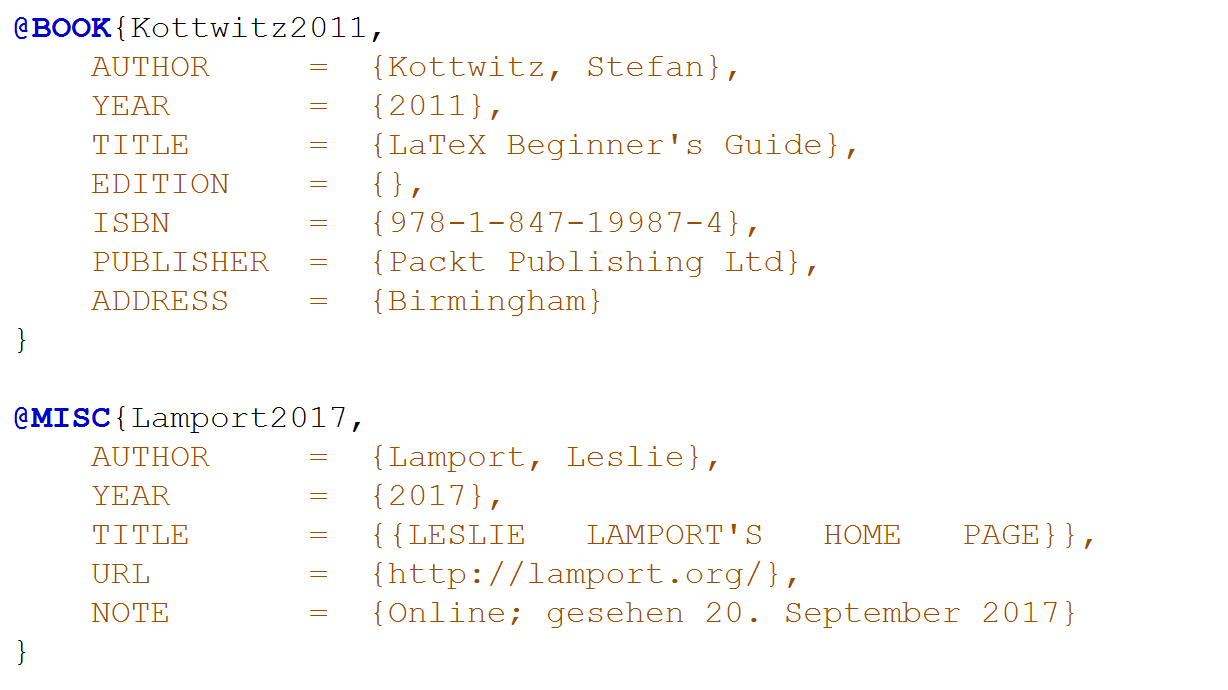
\includegraphics[width=0.75\textwidth]{./Bilder/QuellenErfassen.png}        % Bild ohne Rahmen
  \fbox{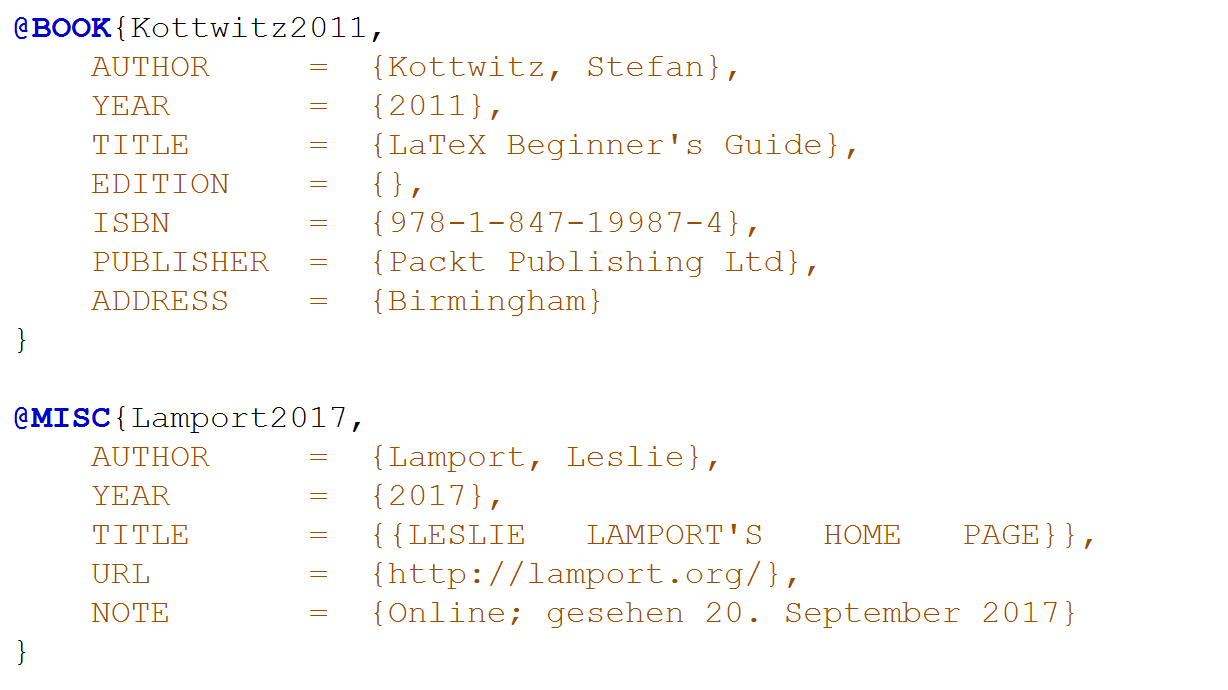
\includegraphics[width=0.75\textwidth]{./Bilder/QuellenErfassen.png}}   % Bild mit Rahmen
  \caption{Erfassen der Quellen}
  \label{fig:QuellenErfassen}
\end{figure} 

Auf der Internet-Seite \menu{\url{http://literatur-generator.de/}} kann man sich solche Einträge generieren lassen.
